% ===============================================================================
\section{Overview}
In this section, we describe how \wingj can be used to detect and model the morphology or structure of a biological system of interest (organ system or body system) from a stack of confocal fluorescence images. The algorithms implemented and their options are also briefly introduced. For detailed information about the methods we developed, please refer to our paper and its Supplementary Notes \autocite{schaffter2013}.\\

In the subsequent sections, a \textit{structure model} of the \droso wing pouch is generated for illustration purpose. The term \textit{structure detection} refers to the process of generating a parametric model describing accurately the morphology of a given system. The structure of the wing pouch is defined by the \emph{outer boundary} (or contour) of the pouch (delimited by the expression of Wingless) inside which the \textit{A/P and D/V compartment boundaries} are detected and segmented from Patch (Ptc) and Wingless expression, respectively. A second biological system supported in \wingj is the \droso embryo. The structure of the embryo is defined as its ellipse-like contour, and the A/P and D/V compartment boundaries that are defined as the axes of the identified contour (\figref{fig:wingj_embryo_detection_modules}). For the detection of the embryo structure, any proteins that are expression more or less everywhere in the embryo (e.g. \textit{eve} or \textit{kr\"{u}ppel} proteins even if their expression is stronger along a few stripes) or localized along the embryo contour can be used.

% ===============================================================================
\section{Opening stacks of confocal images} \label{sec:structure_image_loading}
In \sectionref{sec:open_images}, we explain how to select and open single images or stacks of confocal images in \wingj. Here, we import confocal images where the expression of Wingless and Patch is labelled using a fluorescent dye (Wg-Ptc-AB). As a remainder, we use the expression of Wg-Ptc to make the structure of the \droso wing pouch visible as required for enabling its segmentation\autocite{schaffter2013}.\\

We recommend to use the first channel in \wingj (channel 0) to import Wg-Ptc images because this channel is selected by default to provide the input image for structure detection and is identified by the radio button checked on the left side of the interface (\figref{fig:wingj_interface}). The projection method selected for the default structure channel is also set to \emph{Maximum intensity projection} (\sectionref{sec:structure_projections}), which is the best method for visualizing the structure of a system (\sectionref{sec:structure_automatic}).\\

Stacks of confocal images imported in \wingj are immediately made visible in a new window. To illustrate the use of \wingj in the subsequent sections, we load the images associated to the channel "ch02" from the experiment \textit{20100716\_pmadAB\_brkAB\_wg-ptcAB\_90,5-91,5H\_M\_1}.\footnote{The images of this experiment are included in the \wingjBenchmarkImages.} Use the \emph{mouse wheel} or the horizontal scroll bar at the bottom of the window to navigate through the image slices. Information such as the number of slices in the stack or the resolution of the images is displayed above the images.\\

% Figure~\ref{fig:wingj_import_wg-ptc} shows the window that appears after importing a stack of Wg-Ptc-AB images, here obtained from imaging a 114h-hour-old wild type \textit{Drosophila} wing disc.

% \begin{figure}[!h]
% \centering
% 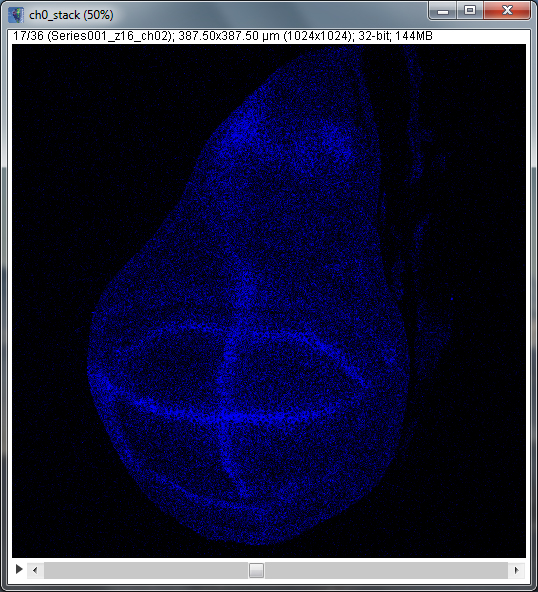
\includegraphics[scale=0.5]{images/wingj_import_wg-ptc_2.jpg}
% \caption{Stacks of images imported in \wingj are immediately made visible in a new window. Here we loaded the channel ch02 associated to Wg-Ptc-AB from the experiment \textit{20100716\_pmadAB\_brkAB\_wg-ptcAB\_90,5-91,5H\_M\_1}. This experiment can be found in the \wingj \wingjBenchmarkImages. Use the mouse wheel or the horizontal scroll bar at the bottom of the window to navigate through the image slices. Information such as the number of slices in the stack or the resolution of the images is displayed above the images.}
% \label{fig:wingj_import_wg-ptc}
% \end{figure}

\textbf{Important}: More detailed information about the protocol we use for wing sample collection, immunostaining, and image acquisition is available in the \textbf{Supplementary Notes} of our paper\autocite{schaffter2013}.

% ===============================================================================
\section{Defining channel names} \label{sec:structure_convention_experiment_channel_names}
As described in \sectionref{convention_experiment_channel_names}, each channel should be named to distinct one from another without ambiguity. The names of the channels are also used to define the names of the files generated by \wingj. \wingj provides a text field for each channel in order to name them.

% ===============================================================================
\section{Setting minimum and maximum z-slice indexes}\label{sec:structure_slice_index}
When importing a stack of confocal images (also called \emph{z-stack}, \textit{Browse $>$ Select images folder}), a dialog appears and reports how many image files are included in the selected images folder. There you can specify the index of the minimum and maximum slices to load as mentioned in \sectionref{sec:open_images}.\\

Moreover, and once an image stack has been imported in \wingj, the index of the minimum and maximum slices to consider can be changed at any time via the main interface. To give an example, dad-GFP is expressed in large spots in the peripodial membrane of the \droso wing. For restrain the quantification of dad-GFP expression to the wing pouch, the image slices corresponding to the peripodial membrane should be removed. This can be achieved by increasing the index of the first slice or by decreasing the index of the last slice depending on the $z$ orientation of the wing. To check that the slices corresponding to the peripodial membrane have been successfully removed, click on \textit{Max} to compute and display the maximum intensity projection in order to verify that the large spots of dad-GFP expression were removed.

% ===============================================================================
\section{Selecting projection method}\label{sec:structure_projections}
A \textit{maximum intensity projection (MIP)} is an image whose pixels contain the maximum value over all images in the stack at the particular pixel location. Similarly, a \textit{mean or average intensity projection} is an image whose pixels contain the average value over all images in the stack at the particular pixel location. \figureref{fig:projection_mean_max} shows the the mean and maximum intensity projections computed from the same image stack.\\

\begin{figure}[!h]
\centering
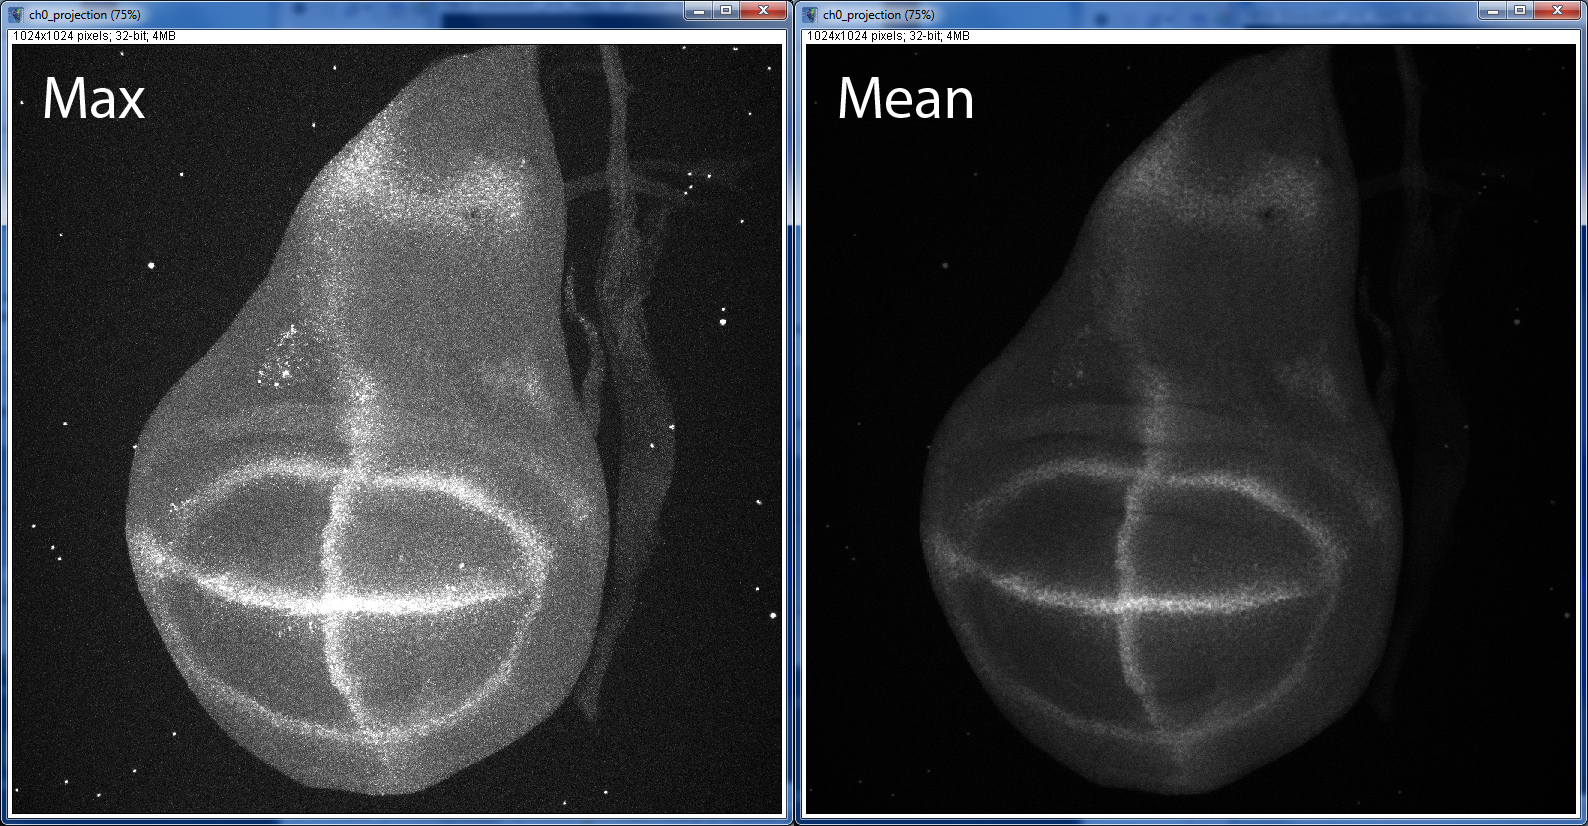
\includegraphics[scale=0.26]{images/projection_mean_max.jpg}
\caption{\textbf{Maximum and average expression maps.} A maximum intensity projection (MIP) is applied to Wg-Ptc confocal images to produce the image that will be used as input for detecting and modeling the structure of the \droso wing. Mean intensity projections are usually computed for quantifying gene and protein expression.}
\label{fig:projection_mean_max}
\end{figure}

MIP are typically used to reveal high concentration of fluorescence in the XY space independently of the $z$ location. Thus, MIP images are particularly suitable for segmenting the structure of the \droso wing pouch. In \wingj, mean intensity projections are used as input for quantifying expression.\\

Click on the \textit{Max} or \textit{Mean} button to select the projection method to use for a given channel and display it. The projection is computed using only the slices included in the range defined by the index of the first and last slices (\sectionref{sec:structure_slice_index}).

% ===============================================================================
\section{Image scale}\label{sec:structure_image_scale}
The relation between \px and \mum, for instance, is extracted automatically by \wingj from the meta-information encoded in the input images. This information is included by the microscope software (we use \textit{Leica Application Suite}).\footnote{\leicaWebsite}\\

If this information is not encoded in your images, edit the parameters \textit{unit} and \textit{scale} in the settings of \wingj (by default 1 \px = 1 \mum). The relation linking \px and \mum is used to export structure and expression datasets in meaningful physical units (e.g. boundary lengths in \mum or compartment areas in \mumsquare).

% ===============================================================================
\section{Defining an area of interest (AOI)}\label{sec:aoi}
The stack of confocal images imported in \wingj may include more than one wing disc or embryo. An \textit{area of interest (AOI)} (also called \textit{region of interest (ROI)}) can be defined to tells \wingj what part of the image data it should consider. \figurerefsub{fig:aoi}{A} shows an example where four wing discs have been imaged at the same time.\\

\begin{figure}[!h]
\centering
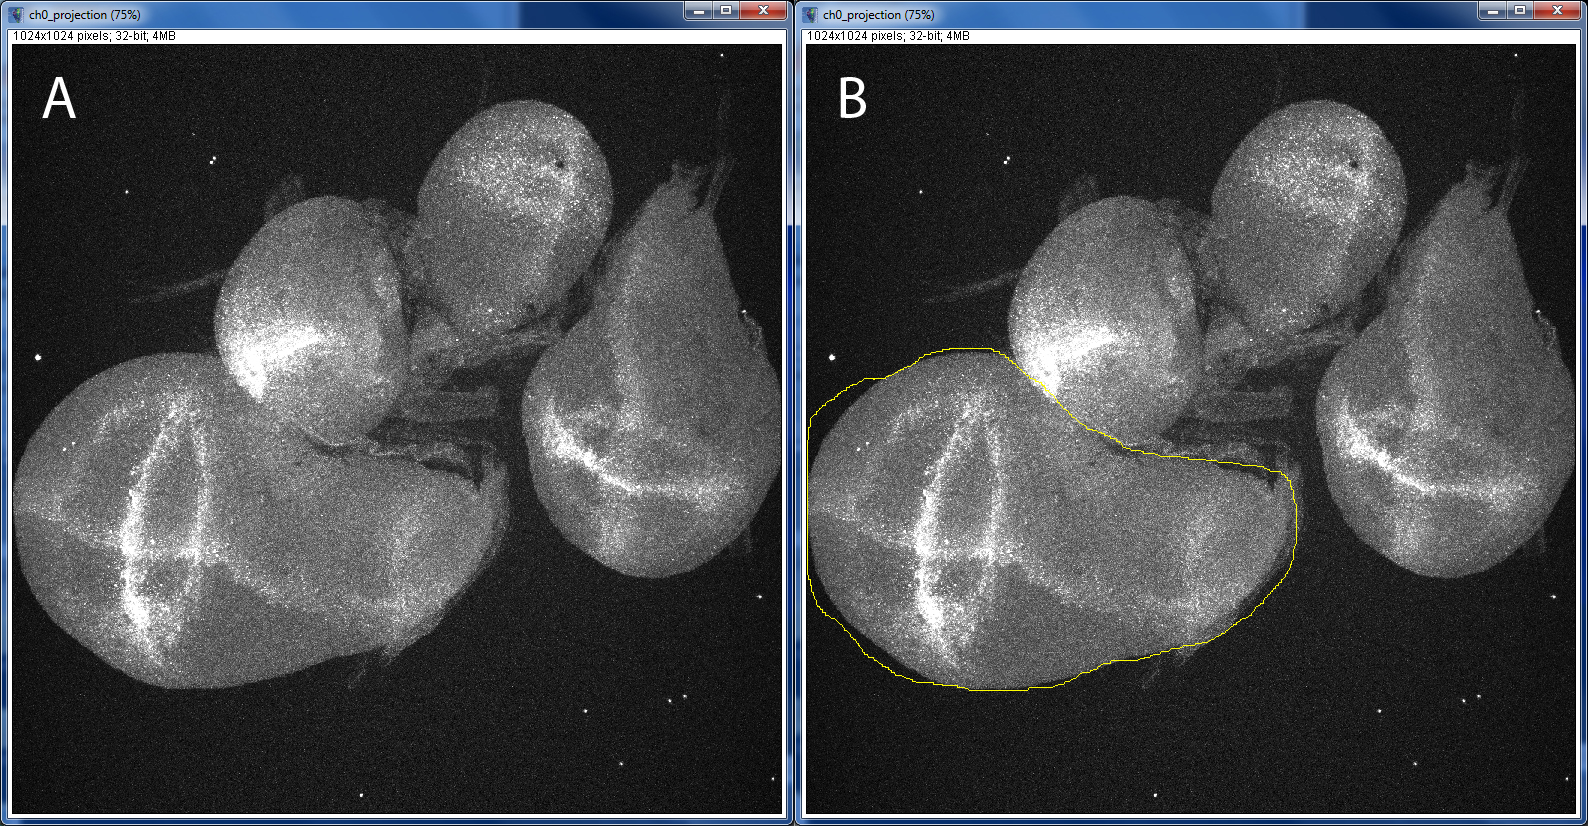
\includegraphics[scale=0.26]{images/aoi.jpg}
\caption{\textbf{Definition of an area of interest (AOI).} (A) Example where four wing discs have been imaged at the same time. (B) An area of interest has been defined to discard any image information outside of this area (here delimited by a yellow polygon).}
\label{fig:aoi}
\end{figure}

To define an area of interest, click on the button \textit{Set AOI}. A new image window appears which shows the projection of the structure channel. The \ij tool \textit{Freehand selections} is then automatically selected from the \textit{\ij toolbar}. To set an AOI, draw a closed polygon around the wing disc to conserve (keep the left button of the mouse pressed while drawing). Click outside of the AOI to remove it. \figurerefsub{fig:aoi}{B} shows an AOI defined to mask part of the image.  Moreover, avoid closing the image window where you defined the AOI as closing this window would result in deleting the AOI.\\

\textbf{Important}: The unsupervised structure detection method we developed for detecting and modeling the morphology or structure of the \droso wing pouch requires at some point to compute the \emph{center of mass} of the wing disc. The center of mass is computed using the pixel values inside the AOI or from the entire projection image if no AOI is defined. Thus it is important that 1) a wing disc is imaged entirely and 2) that the AOI (if required) follows properly the contour of the wing disc and not only the contour of the wing pouch. Note that the center of mass of the wing disc is only used to infer the orientation of the wing pouch and do not participate to the shape of the structure model. Furthermore, the orientation of the model can always be edited later (\sectionref{sec:wingj_structure_edit}).\\

\textbf{Tip}: Try to avoid closing manually the image windows opened by \wingj, for example by clicking on the close button of a window. Instead, let \wingj close the windows which are not required anymore. You may also click on the button \textit{Reset} from the main interface to close all windows opened for the current experiment (also reset the structure detector).

% ===============================================================================
\section{Resetting experiment}
Click on the button \textit{Reset} to close all the windows related to the current experiment and reset internal variables to make \wingj ready for quantifying the next system.

% ===============================================================================
\section{Important settings for \droso wing detection}
Our methods were designed to be robust to many parameter values so that users don't have to spend too much time tweaking parameters for every single experiment.\\

Nevertheless, we recommend that you consider setting the following parameters from the \textit{Settings} panel the first time you run \wingj. \textit{A priori} knowledge about the system to quantify (organ system or body system) increases the success rate of the structure detection method as well as the accuracy of the generated structure models themselves. If the intrinsic properties of the confocal images imported in \wingj are consistent across many experiments, the same parameter values can be reused.

\begin{itemize}
 \item \textbf{expectedBoundariesThicknessInPixels} (\droso wing pouch only). Expected thickness in \px of the fluorescence expressed along the A/P and D/V compartment boundary. To measure the thickness in \px, select the \textit{Straight line} tool from the \textit{\ij toolbar} and draw a line across one of the boundaries. Then click on \textit{\ij toolbar $>$ Analyze $>$ Measure} to get the length of the line in \px.
 \item \textbf{boundaryTrackerNumSteps} (\droso wing pouch only). The product of \textit{boundaryTrackerStepSizeInPixels} and this parameter should be larger than half the length of the longest boundary (A/P or D/V). Set the value of \textit{boundaryTrackerNumSteps} to satisfy this requirement.
 \textit{numStructureControlPoints}. The level of accuracy that a structure model can achieve depends on the number of \emph{control points} per segment used to build the model. Larger numbers of control points allow to enable the generation of more precise models. This parameter should be set depending on the complexity of the structure of the biological system to model. For instance, three to five control points per segment are typically enough for modeling the wing pouch and embryo structure.
 \item \textbf{scale} and \textbf{unit}. This parameter is usually set by \wingj after loading a stack of confocal images. If the input images do not encode this information, set \textit{scale} so that 1 \px = \textit{scale} \textit{unit}. Set the parameter \textit{unit} with one of the following strings: "nm", "um", "micron", "mm", "cm", "meter", "km" or "inch".
\end{itemize}

% ===============================================================================
\section{Pre-processing} \label{sec:pp_parameters}
The select structure detection method may implement a pre-processing stage. Before starting any structure detection by clicking on \textit{Run Detection} or \textit{Step}, (\sectionref{sec:structure_controls}), click on \textit{Pre-Process}.\\

During the pre-processing of the \droso wing pouch, for instance, \wingj performs different operations to find optimal values for a few parameters based on the intrinsic content of the input images. This is done to increase the success rate of the structure detection and increase the accuracy of the structure model generated. Please refer to the \textit{Log window} for detailed information about the pre-processing results.

% Beforehand, you must set the value of the parameter \textit{ppBlur} directly in the settings of \wingj. This parameter corresponds to the standard deviation $\sigma$ of the 2D Gaussian filter applied to remove noise from the maximum intensity projection of the structure image stack. Use the following relation to determine the value of \textit{ppBlur} \autocite{schaffter2013}:
% 
% \begin{equation}
%  \mbox{\textit{ppBlur}} = \frac{\mbox{A/P and D/V boundary thickness in \px}}{2\sqrt{2ln(2)}}
% \end{equation} 
% 
% There is a simple way to measure a distance in \px using the \ij toolbar:
% 
% \begin{enumerate}
%  \item Select the \textit{Straight line} tool from \ij toolbar and draw on top of the Wg-Ptc-AB maximum projection a line reflecting the thickness of the A/P or D/V boundary.
%  \item Click on the menu \textit{Analyze}, then \textit{Measure}.
%  \item The length of the line is given in \px.
% \end{enumerate}
% 
% If this value is consistent across multiple wing pouches (no need to be accurate at the single pixel resolution), this value can be defined once and then used again in multiple experiments.

% \begin{figure}[h!]
% \begin{center}
% \begin{minipage}[b]{0.45\linewidth}
% \centering
% \includegraphics[width=6cm]{figures/structure_step_1_blur_5}
% \end{minipage}
% \hspace{0.5cm}
% \begin{minipage}[b]{0.45\linewidth}
% \centering
% \includegraphics[width=6cm]{figures/structure_step_1_blur_10}
% \end{minipage}
% \end{center}
% \caption{Effect of the parameter \textit{Blur} on the pre-processed image. This parameter corresponds to the standard deviation $\sigma$ in $[px]$ of a 2D Gaussian filter. The pre-processing consists in blurring and the thresholding the projection of the structure image (input). (Left) \textit{Blur} = 5. (Right) \textit{Blur} = 10 for a better result.}
% \label{fig:structure_step_1_blur}
% \end{figure}

% It has been observed that the parameter \textit{Blur} is robust and that its value can be conserved across several experiments if the fluorescence intensity do not change drastically from one experiment to another. Therefore for future experiments, setting the pre-processing parameters is as simple as clicking on \textit{Auto} to adjust automatically the value of \textit{Threshold}. Fig. \ref{fig:structure_step_1_threshold} shows the effect on the pre-processed image of different values for \textit{Threshold}.

% \begin{figure}[h!]
% \begin{center}
% \begin{minipage}[b]{0.45\linewidth}
% \centering
% \includegraphics[width=6cm]{figures/structure_step_1_thres_65}
% \end{minipage}
% \hspace{0.5cm}
% \begin{minipage}[b]{0.45\linewidth}
% \centering
% \includegraphics[width=6cm]{figures/structure_step_1_thres_75}
% \end{minipage}
% \end{center}
% \caption{Effect of the parameter \textit{Threshold} on the pre-processed image. After blurring, pixels with values lower than \textit{Threshold} are set to 0 (black), otherwise 255 (white). (Left) \textit{Threshold} set to 65. (Right) \textit{Threshold} set to 140 to obtain a clearer visualization of the wing pouch structure. Note that structure detection method succeeds to delimit the contour of the structure even if the pre-processed structure is broken as it is the case here.}
% \label{fig:structure_step_1_threshold}
% \end{figure}

% ===============================================================================
\section{Structure detection controls}\label{sec:structure_controls}
The main interface of \wingj includes several buttons for running and interacting with structure detections (\figref{fig:structure_detection_buttons}). We give below a description for each control:\\

\begin{figure}[!h]
\centering
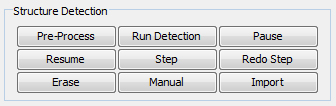
\includegraphics[scale=0.8]{images/structure_detection_buttons.jpg}
\caption{\textbf{Structure detection controls.} The main interface of \wingj includes many buttons to intuitively interact with structure detections.}
\label{fig:structure_detection_buttons}
\end{figure}

\begin{itemize}
 \item \textbf{Run Detection}. Starts the detection and modeling of the selected system while requesting as less interactions as possible from the user (\sectionref{sec:structure_automatic}). A structure detection is composed of multiple \textit{detection modules}, each being designed to identify a specific feature of the overall structure to model (see \sectionref{sec:wpouch_class_diagram} for a description of each of the modules applied to infer the structure of the wing pouch). Don't forget to select the system to model (\sectionref{sec:biological_system}) as the detection modules applied would be different from one structure detection method to another.

 \item \textbf{Pause}. Pauses the structure detection. The detection can be resumed by clicking on \textit{Resume}, or \textit{Step} to continue in step-by-step mode.

 \item \textbf{Resume}. Resumes the structure detection previously paused or performed so far in step-by-step mode.

 \item \textbf{Step}. Performs one step of the current structure detection. A single detection module is applied each time the button \textit{Step} is pressed (\sectionref{sec:supervised_structure}).

 \item \textbf{Redo Step}. Redoes the last step of the structure detection. This feature is useful to evaluate the output of a detection module obtained when different values of a parameter are used.

 \item \textbf{Erase}. Resets the current structure detection. Click on \textit{Run Detection} to start a new unsupervised detection. Click on \textit{Step} to start a new step-by-step detection. Click on \textit{Manual} to define manually the structure. Click on \textit{Import} to load a \wingj structure model previously saved to file.

 \item \textbf{Manual}. Provides tools to manually define a structure model starting from a generic structure shape (\sectionref{sec:manual_detection}).

 \item \textbf{Import}. Loads a structure model previously saved to file (\sectionref{sec:structure_import}).
\end{itemize}

% ===============================================================================
\section{Automatic structure detection}\label{sec:structure_automatic}
\subsection{Overview}
As mentioned above, the structure detection consists in generating a parametric model that accurately describes the morphology or structure of a biological organism (e.g. \droso embryo) or organ (e.g. \droso wing pouch). The approach we developed is based on the design of many \textit{detection modules} that each takes care of identifying a specific feature of the overall structure to model\autocite{schaffter2013}. Examples of the application of detection modules are the detection of specific fluorescent shapes, detection of closed compartments, and identification of the trajectory of fluorescent boundaries.\\

There are mainly two ways to generate a structure models in \wingj: \textit{automatically} or \textit{step by step}. The first method aims to provide a way to generate structure models while requesting as less interactions as possible from the user. The detection of the \droso wing pouch, for instance, takes as input Wg-Ptc images and generates a complete model of the structure of the pouch in an unsupervised way before showing it to the user for validation. Once the structure has been validated, an algorithm we developed infers automatically the A/P and D/V orientation of the wing in the image space. Thus if no manually fine-tuning are required, the detection of the wing pouch takes as much as three clicks (\textit{Pre-Process}, \textit{Run Detection}, and validation of the structure). In the next section, we describe in more details how to run automatic structure detections.\\

\textbf{Tip}: \wingj provides tools to manually model the structure of an organ or body system, for instance when a structure detection algorithm has not yet been implemented for the biological system considered. After loading the required stack of images, click on \textit{Manual} from the main interface of \wingj to generate a generic structure model that can then be shaped to match any structure (\sectionref{sec:manual_detection}).

% ===============================================================================
\subsection{Requirements} \label{sec:unsupervised_detection_guidelines}
To profile the performance of our structure detection method, we defined a 50-wing benchmark and reported the success rate of the detection modules whose output consistency is crucial for the generation of structure models \autocite{schaffter2013}. The success rate is computed by comparing the output of a detection module to a \textit{ground truth} obtained manually. In particular, we assessed the performance of the detection module whose task is to identify the intersection of the A/P and D/V compartment boundaries for different parameter values. From those experiments, we can list a few guidelines to improve the accuracy and robustness of the wing pouch structure detection.

\begin{itemize}
 \item \textbf{Align the A/P and D/V compartment boundaries with the borders of the image} (\droso wing pouch only). The fluorescent cross-like shape made by the expression of Wg-Ptc along the A/P and D/V boundaries should be oriented like a plus sign '+' in the image canvas. This constraint comes from the fact that we use a simple method to identify the intersection of the A/P and D/V boundaries based on the projection of the image pixels on the $x$- and $y$-axis of the image. Note that it doesn't matter whether the A/P boundary is parallel to the $x$- or $y$-axis of the image. The correct orientation is inferred later based on prior information about the morphology of the wing (\sectionref{sec:orientation_inference}). In the \textbf{Supplementary Notes} of our paper, we report that deviations of about $\pm8$\degree still allow the detection module to successfully and automatically identify the intersection of the A/P and D/V boundaries \autocite{schaffter2013}. In the near future, we wish to replace this detection module by a new one that would be able to identify a fluorescence cross-like shape independently of its orientation.

 \item \textbf{Define an area of interest}. An AOI should be defined whenever more than one wing or embryo, for instance, are visible in the same stack of confocal images.

 \item \textbf{Remember to click on \textit{Pre-Process}}. The pre-processing method, which depends on the selected system detection method, sets many parameters with optimal values based on the intrinsic content of the input images in order to increase the success rate of the structure detection. If required, the parameter values set by the pre-processing method can still be overridden in the settings before starting the structure detection. See the content of the \textit{Log window} to know which parameters are being optimized.
\end{itemize}

% ===============================================================================
\subsection{Running detection}
Click on \textit{Pre-Process}, then click on \textit{Run Detection} to automatically detect and infer a model of the structure of the wing pouch or the embryo.\\

\textbf{Tip}: To supervise the automatic structure detection if it came to fail, click on \textit{Erase} to reset the detection method, then click on \textit{Step} to run the structure detection step by step and thus obtain insight into why the structure detection failed (\sectionref{sec:supervised_structure}).

% ===============================================================================
\section{Editing the shape of structure models}\label{sec:edit_structure_before_validation}
The structure model inferred is then shown on top of the input image projection (\figrefsub{fig:wingj_structure_detection}{A}).

\begin{figure}[!h]
\centering
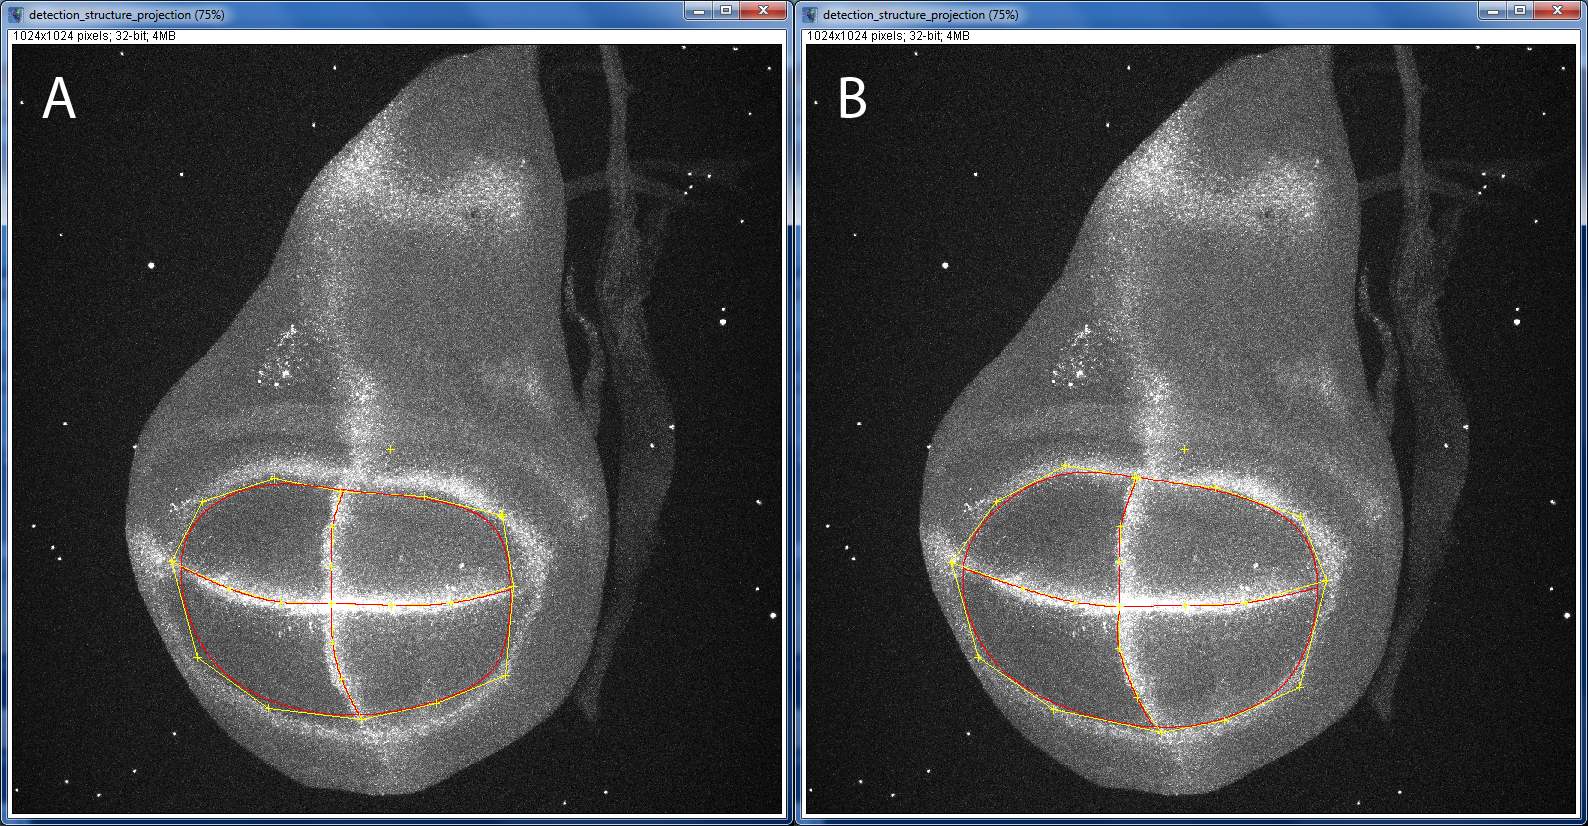
\includegraphics[scale=0.26]{images/wingj_structure_detection.jpg}
\caption{\textbf{Interactive structure model generated by \wingj from the Wg-Ptc confocal images.} (A) Visual representation of the parametric model automatically generated by \wingj. The relevant structure is defined by the red, smooth polygon. The \emph{control points} of the model are represented as by yellow vertices '+'. (B) \wingj provides tools to fine-tune the structure models identified. In our experiments, we make the structure model fit the expression of Wg-Ptc as shown. Mainly, the contour of the model should fit the inner contour of the wing pouch and the model of the A/P compartment boundary should follow the expression of Patch (Ptc) on the posterior side (here on the left). Finally, the D/V compartment boundary should be centered on the expression of Wg.}
\label{fig:wingj_structure_detection}
\end{figure}

The relevant structure is defined by the red, smooth polygon. The \emph{control points} of the parametric model are represented as by yellow vertices '+'. The shape of the structure can be modified by moving around the control points of the model. To validate the model, for instance having fine-tuned the structure if required (\figrefsub{fig:wingj_structure_detection}{B}), click on the \textit{tick mark} from the \textit{\ij toolbar} (\figref{fig:ij_toolbar}). Before that, \wingj changed the content of the \textit{\ij toolbar} to provide tools to help visualizing and editing the structure model. From left to right in the \textit{\ij toolbar}:

\begin{figure}[!h]
\centering
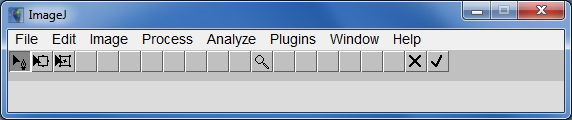
\includegraphics[scale=0.6]{images/ij_toolbar.jpg}
\caption{\textbf{Tools proposed by \wingj to visualize and edit structure models.} Before validating a structure model, \wingj modifies the content of the \textit{\ij toolbar} to include tools to edit the structure model (translation, rotation, scaling, etc.). Click on the \textit{tick mark} to validate the model and the infer the orientation of the model (\sectionref{sec:orientation_inference}).}
\label{fig:ij_toolbar}
\end{figure}

\begin{itemize}
 \item \textbf{Move crosses}. Move individual control points '+'. The control points are the parameters of the model and define the shape of the structure model. If you click somewhere in the image, the closest control point will be selected. If the mouse cursor moves slightly while being clicked, the selected control point will jump to the location of the mouse cursor. Hold \textit{Shift} to move the entire structure.
 \item \textbf{Resize snake}. Hold \textit{Shift} to resize the structure model while conserving the ratio between its dimensions. Otherwise the width and height of the model can be independently resized.
 \item \textbf{Rotate snake}. Click somewhere on the image and move the mouse cursor to rotate the model.
 \item \textbf{Magnifying glass}. Left/right click on the image to zoom in/out.
 \item \textbf{Abort}. Click on the cross mark to abort the edition of the structure model.
 \item \textbf{Accept}. Click on the tick mark to validate the structure model.
\end{itemize}


% \begin{figure}[h!]
% \centering\includegraphics[width=12cm]{figures/structure_runall}
% \caption{After having successfully identified the structure of the \textit{Drosophila} wing, WingJ displays the output, which can be edited by moving the vertices (small yellow crosses). Press MAJ key to drag-and-drop the entire structure.}
% \label{fig:structure_runall}
% \end{figure}

% \begin{figure}[h!]
% \centering\includegraphics[width=8.2cm]{figures/imagej_bar}
% \caption{WingJ provides tools to fine-tune the identified structure. From left to right: \textit{move crosses}, \textit{resize}, \textit{rotate}, and \textit{magnifying glass}. Click on the \textit{Cross mark} button to reject the structure, or on the (\textit{Tick mark} to validate it.}
% \label{fig:imagej_bar_detection}
% \end{figure}

% ===============================================================================
\section{Inferring the orientation of the structure model}\label{sec:orientation_inference}
The task of the remaining detection module is to infer the orientation of the structure model in the image space. Concretely for the \droso wing and embryo, the orientation inference consists in identifying the A/P and D/V directions and thus label their four compartments DA, DP, VA, and VP respectively.\\

The inference of the orientation of the wing pouch is based on the curvature of the A/P and D/V compartment boundaries identified and the center of mass of the wing disc (\figref{fig:wingj_orientation}). Among the four points that connect the A/P and D/V boundaries to the outer boundary (or contour) of the wing pouch, the point D is defined as the closest point to the wing disc center of mass. That's why it is important that the free yellow vertex '+' representing the center of mass of the wing disc is placed near the effective point D before validating the structure model (\sectionref{sec:edit_structure_before_validation}). This should already be the case if the wing disc has been entirely imaged and/or an area of interest has been properly defined. Knowing the dorsal direction (point D) means knowing the anterior side and so the orientation of the A/P boundary (D-V axis).\\

The orientation of the D/V boundary is obtained from the observation that the exterior of the curves made by the A/P and D/V boundaries point towards the posterior and ventral side, respectively. The details of the algorithm we developed to infer the orientation of the wing pouch are given in the \textbf{Supplementary Notes} of our paper \autocite{schaffter2013}.

\begin{figure}[!h]
\centering
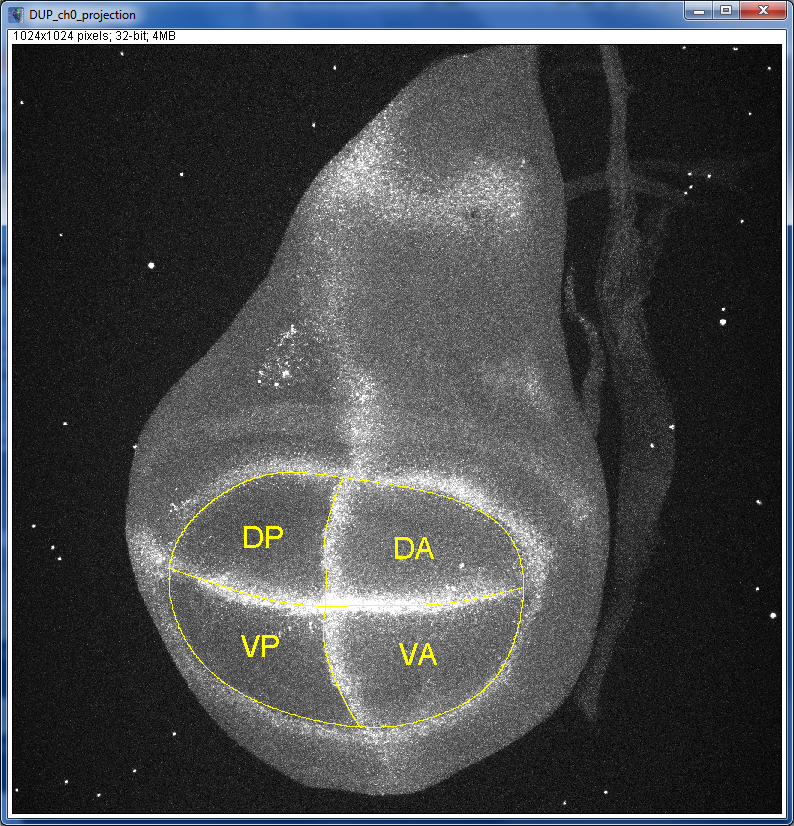
\includegraphics[scale=0.35]{images/wingj_orientation.jpg}
\caption{\textbf{Unsupervised A/P and D/V orientation inference of the \droso wing.} Here, the structure model inferred is automatically displayed on top of the Wg-Ptc projection once the structure detection is done. Furthermore, the identity of each compartment DA, DP, VA, and VP is revealed after the orientation inference.}
\label{fig:wingj_orientation}
\end{figure}

For the \droso embryo, \wingj asks the user to indicate where is the dorsal-anterior compartment to enable the identification of the three remaining compartments. One approach to obtain an unsupervised orientation inference would be to identify a gene that is asymmetrically expressed inside the embryo along the A/P and D/V boundaries. One solution could be to label the expression of the \textit{hairy} protein using a fluorescent dye. The A/P and D/V compartment boundaries can be easy differentiated as the D/V boundary is the longest one.

% A possibility could be to use the \textit{hairy} protein (in red in Fig.~\ref{fig:embryo_hairy}).

% \begin{figure}[!h]
% \centering
% 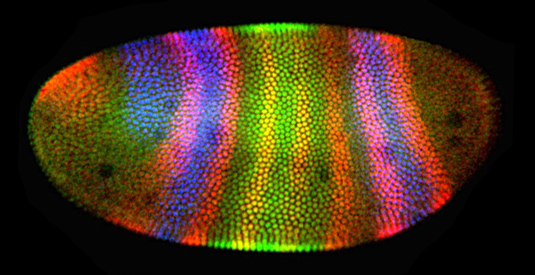
\includegraphics[scale=0.4]{images/embryo_hairy.jpg}
% \caption{The \textit{hairy} protein (in red) is asymmetricly expressed in the embryo and thus could be used to distinct the anterior (left)/posterior and dorsal (top)/ventral orientations. A similar approach will most likely be implemented in a future release of \wingj.}
% \label{fig:embryo_hairy}
% \end{figure}

% ===============================================================================
\section{Structure panel}\label{sec:structure_panel}
% ===============================================================================
\subsection{Overview}
The \emph{Structure panel} is then displayed once the structure model is complete. As a reminder, a structure model is a parametric model used to describe the morphology or structure of a biological organism (e.g. \droso embryo) or organ (e.g. \droso wing pouch). The \emph{Structure panel} gathers tools to interact with this model and provides options to export structure datasets (\figref{fig:wingj_orientation}).

\begin{figure}[!h]
\centering
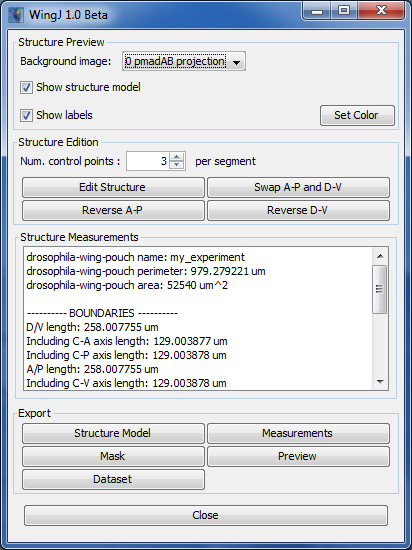
\includegraphics[scale=0.6]{images/wingj_structure_panel.jpg}
\caption{\textbf{Structure panel.} The \emph{Structure panel} is displayed once the structure model is complete. It comes along with a preview of the structure model as shown in \figureref{fig:wingj_orientation}. The \textit{Structure panel} includes tools to edit the inferred model (\sectionref{sec:wingj_structure_edit}), reports measurements taken from the model (\sectionref{sec:wingj_structure_measurements}) and enables to export structure datasets (\sectionref{sec:wingj_structure_dataset}). Click on \textit{Close} to go back to the main interface of \wingj. From there, click on \textit{Structure} to return to this panel.}
\label{fig:wingj_structure_panel}
\end{figure}

% ===============================================================================
\subsection{Structure viewer}
The \emph{structure viewer} is shown as long as the \textit{Structure panel} is displayed. The viewer displays many elements as shown in \figureref{fig:wingj_orientation}.

\begin{itemize}
 \item \textbf{Background image}. Selects the background image to display from the list. The list includes the stacks of confocal images opened in \wingj (if selected, hold the mouse cursor on top of the viewer and use the mouse wheel to navigate through the slices) and their respective projections, which takes into account the index of the minimum and maximum z-slices specified.
 \item \textbf{Structure model}. Checks this option to display the structure model on top of the background image.
 \item \textbf{Labels}. Checks this option to display additional information such as the name of the compartments included in the structure model.
\end{itemize}

% ===============================================================================
\subsection{Editing the shape and orientation of structure models}\label{sec:wingj_structure_edit}
The \emph{Structure panel} provides tools to edit the current model. Click on \textit{Edit} to modify the shape of the structure model. The number of control points per segment can be increased to fit more complex structure shapes. The number of control points can be increased or decreased at any time from the \emph{Structure panel}. \figureref{fig:wingj_structure_control_points} shows two models obtained when using three and five controls points per segment.

% However the higher the number of control points is, the more time it can take when it come to manually modify the structure model.

\begin{figure}[!h]
\centering
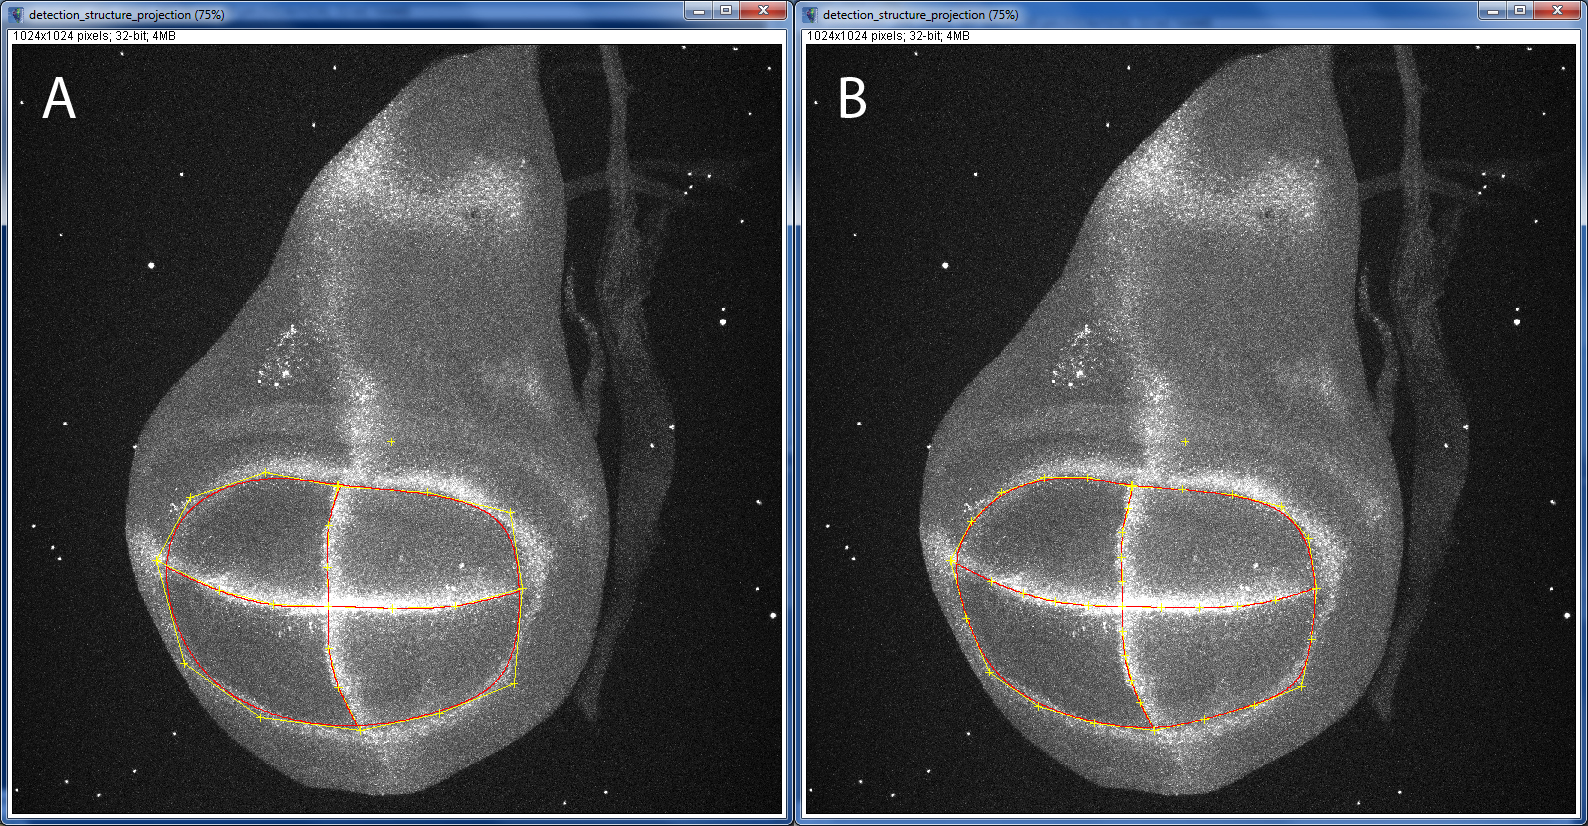
\includegraphics[scale=0.26]{images/wingj_structure_control_points.jpg}
\caption{\textbf{Effect of the number of control points on the shape of structure models.} The number of \textit{control points} of the parametric structure model can be increased or decreased at any time from the \textit{Structure panel}. The number of control points is specified per segment and the default number of control points can be changed in the settings of \wingj. Here, the structure models reported have (A) three and (B) five control points per segment.}
\label{fig:wingj_structure_control_points}
\end{figure}

As described in \sectionref{sec:orientation_inference}, the structure detection method we developed for the \droso wing automatically infers the orientation of the wing in the space of the image. In case the orientation inferred is not correct, the following buttons can be used to edit the orientation of the model:

\begin{itemize}
 \item \textbf{Swap A-P and D-V}. Swaps the identity of the current anterior-posterior and dorsal-ventral axes. Note that the A-P axis corresponds to the D/V compartment boundary and that the D-V axis corresponds to the A/P compartment boundary.
 \item \textbf{Reverse A-P}. Reverses the direction of the anterior-posterior axis.
 \item \textbf{Reverse D-V}. Reverses the direction of the dorsal-ventral axis. 
\end{itemize}

% ===============================================================================
\subsection{Structure measurements}\label{sec:wingj_structure_measurements}
The text box included in the \textit{Structure panel} reports measurements taken from the structure model. The content may be different depending on the biological system selected (\sectionref{sec:biological_system}). For the wing pouch, measurements include the length of the A/P and D/V boundaries, the length of the four \textit{half-boundaries} that make the A/P and D/V boundaries (C-A, C-P, C-V and C-D, where the point C is the intersection of the A/P and D/V boundaries), the perimeter and area of each of the four compartments DA, DP, VA, and VP, and the area and perimeter of the entire wing pouch.\\

The values are given in meaningful physical units (e.g. \mum or \mumsquare) whenever the input images encode the meta-information about the image scale (otherwise they are given in \px and \pxsquare). If the stack of confocal images used doesn't include this information, go to the \textit{Settings panel} and edit the parameter \textit{scale} and \textit{unit} (\sectionref{sec:structure_image_scale}).

% ===============================================================================
\subsection{Exporting structure datasets}\label{sec:wingj_structure_dataset}
Measurements taken from the structure model can be exported to files from the \emph{Structure panel}. A complete structure dataset includes the following elements:

\begin{itemize}
 \item \textbf{Structure Model}. Exports the structure model to file in a format readable by \wingj. Click on the button \textit{Import} from the main interface of \wingj to load a structure model previously saved to file. Also, three additional text files are saved:
    \begin{itemize}
     \item \textit{my\_experiment\_structure\_A-P.txt}: TSV file (tab separated values) containing the coordinates of the A-P axis (i.e. the D/V boundary) from anterior to posterior. Each line contains the X and Y coordinates of a sample point taken along the A-P axis. The coordinates are given in \px. \textit{my\_experiment} is the name given to the current experiment.
     \item \textit{my\_experiment\_structure\_V-D.txt}: TSV file containing the coordinates of the V-D axis (i.e. the A/P boundary) from ventral to dorsal. Each line contains the X and Y coordinates of a sample point taken along the A-P axis. The coordinates are given in \px.
     \item \textit{my\_experiment\_structure\_contour.txt}: TSV file containing the coordinates of the contour of the structure model. The coordinates are given in \px.
    \end{itemize}
 \item \textbf{Measurements}. Exports structure measurements to file in XML format. The content of this file can be read by the \wingj \matlab toolbox for generating statistics and plots (\sectionref{chap:matlab}).
 \item \textbf{Mask}. Exports a binary image in TIFF format that can be used as mask. Pixels inside the structure model are set to white (pixel value or \textit{brightness} is 255), otherwise black (0).
 \item \textbf{Preview}. Exports the content of the structure viewer as shown in \figureref{fig:wingj_orientation} in TIFF format (useful to visualize quickly how the structure model generated looks like when browsing the experiment folder).
 \item \textbf{Dataset}. Exports the complete structure dataset including each of the above items. In the \textit{Save} dialog that appears, enter a generic filename (without extension). The filename of each file exported will then be based on the given generic filename (e.g. \textit{genericFilename.xml}, \textit{genericFilename\_measurements.txt}, \textit{genericFilename\_mask.tif} and \textit{genericFilename.tif}).
\end{itemize}

% ===============================================================================
\section{Step-by-step structure detection} \label{sec:supervised_structure}
% ===============================================================================
\subsection{Overview}
The generation of structure models can be run step by step to apply a single detection module at a time and visualize its output. Remember to always click on \emph{Pre-Process} before starting a new structure detection. Then click on \textit{Step} multiple times from the main interface of \wingj until the structure model is complete. Click on \textit{Redo Step} to run again the last detection module applied. This feature can be used to test different values of a parameter set in the \emph{Settings panel}. Click on \textit{Resume} to apply the remaining detection modules in an automatic way.\\
% 
% The principal purpose of the step by step detection is to help identifying recurrent issues that may hinder the performance of the automatic structure detection. For example, the effect of the pre-processing parameter \textit{ppBlur} is crutial for detecting the intersection point of the A/P and D/V boundary in the wing pouch. Going step by step allows to check that this point is successfully identified. Most importantly, we expect the quality of the input images to be the principal source of errors (e.g. due to very diffused fluorescence expression). Please refer to the Supplementary Material for the protocol we used to generate Wg-Ptc-AB images \autocite{schaffter2013}.\\

We give below the list of the detection modules applied for generating the structure models of the \droso wing pouch and embryo \autocite{schaffter2013}.

% ===============================================================================
\subsection{\droso wing pouch}\label{sec:wpouch_class_diagram}
\figureref{fig:wingj_wpouch_detection_modules} reproduces the class diagram introduced in the \wingjDeveloperGuide that shows how wing pouch structure detection is performed in \wingj. Detailed information about the algorithms implemented by each detection module is available in the \textbf{Supplementary Notes} of our paper \autocite{schaffter2013}.

\begin{figure}[!h]
\centering
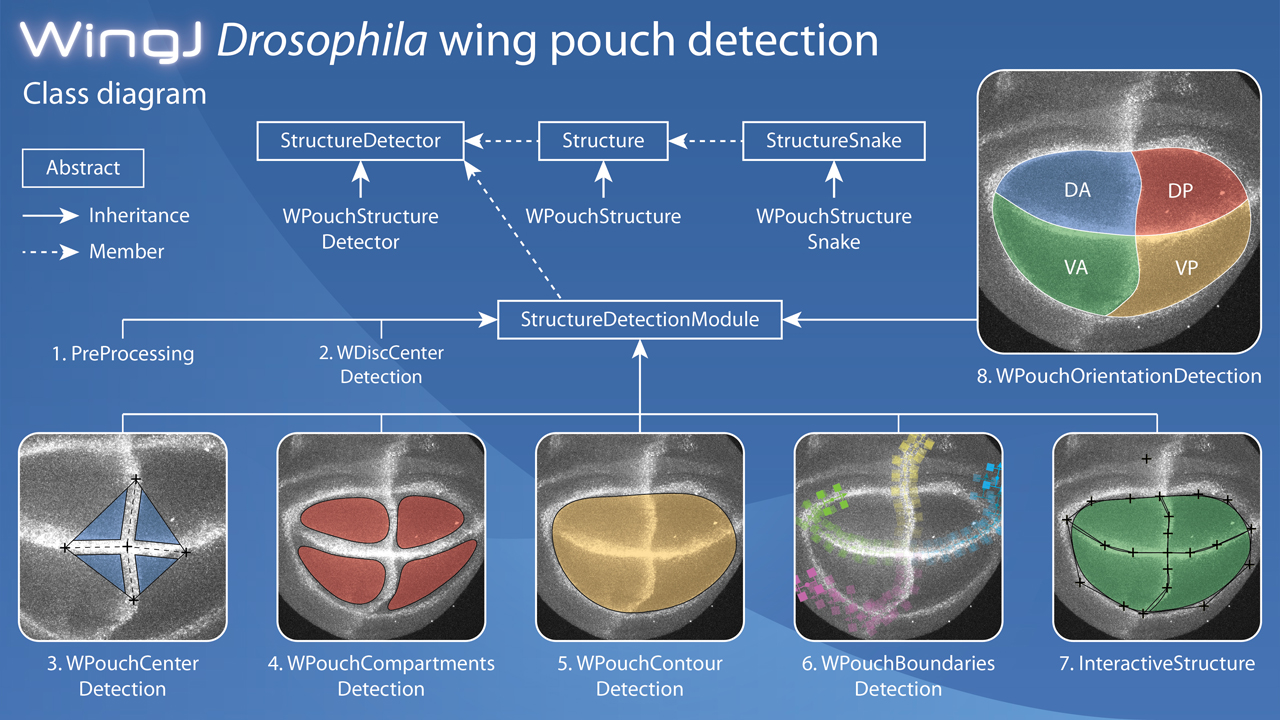
\includegraphics[scale=0.32]{images/wingj-wpouch-diagram-720p.jpg}
\caption{\textbf{Class diagram for detecting and modeling the \droso wing pouch in \wingj.} The detection consists in applying several different \textit{detection modules} that have been designed to identify each a specific feature of the structure. Finally, the outputs of the modules are combined to generate a consistent model of the overall structure of the pouch. This figure is reproduced from the \wingjDeveloperGuide, which provides instructions for extending \wingj to support additional biological systems.}
\label{fig:wingj_wpouch_detection_modules}
\end{figure}

\begin{enumerate}
 \item \textbf{Pre-processing}. Initializes the structure detection method and creates a binary representation of the wing pouch structure used by the next module to identify the intersection of the A/P and D/V compartment boundaries. In the current implementation of \wingj, it is important that the binary structure generated looks in some way like the one shown in \figureref{fig:pp_binary_structure}. Ideally, the A/P and D/V boundaries should form a \emph{straight} cross-like shape, thus it is important that the fluorescence expressed along these boundaries is well visible. Note that the shape of this binary structure depends on the parameters \textit{expectedBoundariesThicknessInPixels} and \textit{ppThreshold}. If the binary structure doesn't match the required shape, go to \textit{Settings}, change the value of \textit{expectedBoundariesThicknessInPixels} then click on the button \textit{Pre-Process} to automatically find a correct value for \textit{ppThreshold}.

\begin{figure}[!h]
\centering
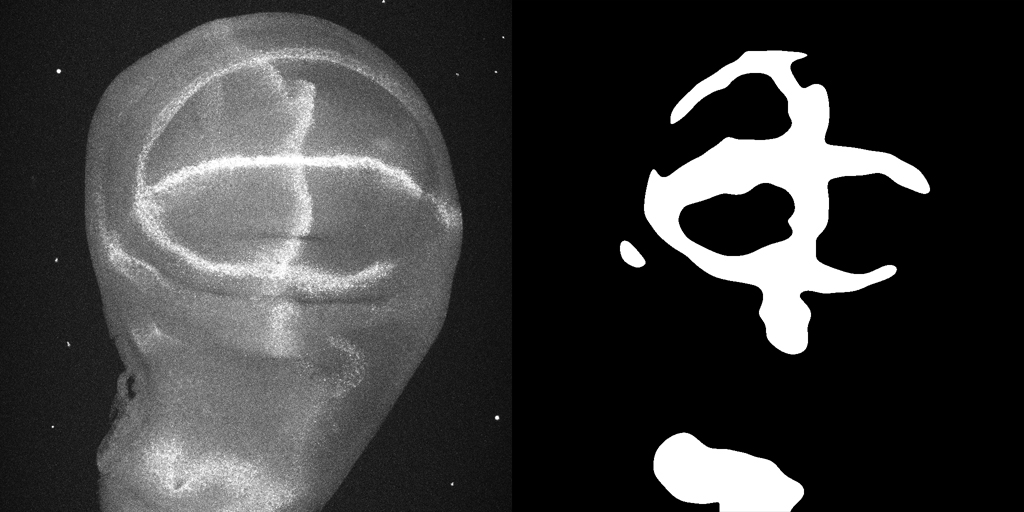
\includegraphics[scale=0.40]{images/pp_binary_structure.jpg}
\caption{\textbf{Pre-processing of the input structure image (projection) to later identify the intersection of the A/P and D/V compartment boundaries.} (Left) Maximum intensity projection of a 100-hour-old \droso wing pouch where its outer boundary and A/P and D/V boundaries are made visble by labelling the expression of Wg-Ptc. It is particularly important that the expression along these boundaries is strong enough for correctly identifying their intersection point. (Right) The image on the left is blurred depending on the expected thickness in \px of the boundaries (parameter \textit{expectedBoundariesThicknessInPixels} in \textit{Settings}). Then, a suitable value for thresholding the blurred image is obtained by clicking on \textit{Pre-Process}. Alternatively, you can set yourself the parameter \textit{ppThreshold} in \textit{Settings} using a value included in [1,255]. Ideally, the binary structure should contain the A/P and D/V boundaries entirely. It is not required for the contour of the wing pouch to be conserved.}
\label{fig:pp_binary_structure}
\end{figure}

 \item \textbf{Detection of the wing disc center (hidden)}. Computes the center of mass of the wing disc. This detection module is run silently even in step by step mode. The output of this module can be visualized and edited when the \emph{interactive structure model} is shown.
 \item \textbf{Detection of the intersection of the A/P and D/V compartment boundaries}. Detects the intersection of the A/P and D/V boundaries by projecting a skeletonized version of the binary structure previously computed on the $x$- and $y$-axis of the image (\sectionref{sec:unsupervised_detection_guidelines}). A key parameter for the correct identification of the A/P and D/V intersection is \textit{expectedBoundariesThicknessInPixels} (\sectionref{sec:unsupervised_detection_guidelines}). Also, the A/P and D/V boundaries are required to be aligned with the $x$- and $y$-axis of the image (\sectionref{sec:unsupervised_detection_guidelines}). Moreover, the arms of the \textit{kite snake} (an optimizer we developed and which has the shape of a kite) must be aligned with each of the four \textit{half-boundaries} that are part of the A/P and D/V boundaries. If this is not the case, the entire structure of the kite snake can be moved by pressing the \emph{Shift} key and the left mouse button. Once the center of the kite snake is align on the intersection of the boundaries, click on the \textit{Play} button (fourth button from the left in the \ij toolbar) to optimize it and align its arms along the fluorescent boundaries. If required, the position of each arm can be edited individually by moving around their respective control point '+'.
 \item \textbf{Detection of the four compartments}. Detects the four compartments DA, DP, VA, and VP included in the wing pouch (their identity will only be unravelled after the inference of the orientation). The robustness of the detection method allows compartments to be simply roughly identified, so there is no need to make them perfectly matching the effective contour of the compartments. A detected compartment can even leak inside another compartment without affecting the output structure model, but it is important that no compartments leak outside of the wing pouch. The snakes can be edited and optimized in a similar way than the kite snake (see above).
 \item \textbf{Detection of the wing pouch contour (hidden)}. Uses the four compartments detected previously to obtain the contour of the wing pouch.
 \item \textbf{Detection of the trajectory of the A/P and D/V compartment boundaries}. Detects the trajectory of the A/P and D/V boundaries using an approach that takes inspiration from line-following robots. The motion of the trackers is shown in step-by-step mode. This motion is slowed down for visualization purpose. The time in seconds between two tracker location updates is defined by the parameter \textit{boundaryTrackerShowDuration} in \textit{Settings}. Also, there are two parameters that can be fine tuned. The first parameter, \textit{boundaryTrackerStepSizeInPixels} determines the step size of the tracker. Too large values wouldn't allow the tracker to follow accurately the fluorescence trajectory (large jumps would make it leave the track) when too small values can make the tracker not going along the desired half-boundary (when the tracker makes its first steps). This parameter value multiplied by the second parameter \textit{boundaryTrackerNumSteps} gives the expected distance covered by one tracker (ideally this value should be around the length in \px of the longest half-boundary). Anyway, only the part of the trajectory that falls inside the pouch is considered, the rest being discarded.
 \item \textbf{Interactive structure model}. Shows the structure model built and provides tools for visualization and fine-tuning. Please refer to the instructions given in \sectionref{sec:orientation_inference} to ensure a successful orientation inference of the wing pouch structure model.
 \item \textbf{Inference of the structure orientation (hidden)}. Detects automatically the A/P and D/V orientation of the wing in the image space. The identity of each of the compartments DA, DP, VA, and VP included in the wing pouch are then unravelled (\sectionref{sec:orientation_inference}).
\end{enumerate}

% ===============================================================================
\subsection{\textit{Drosophila} embryo}\label{sec:embryo_detection}
\figureref{fig:wingj_embryo_detection_modules} reproduces the class diagram introduced in the \wingjDeveloperGuide that shows how embryo structure detection is performed in \wingj. Detailed information about the algorithms implemented by each detection module is available in the \textbf{Supplementary Notes} of our paper \autocite{schaffter2013}.

\begin{figure}[!h]
\centering
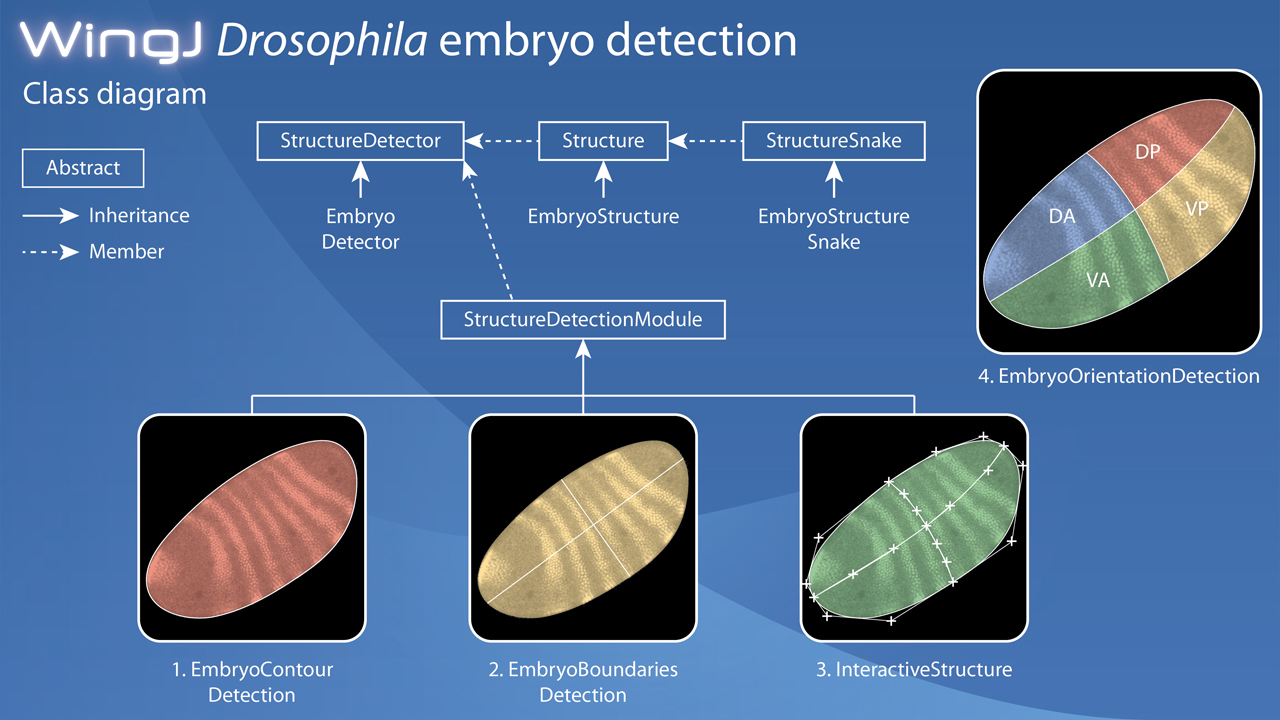
\includegraphics[scale=0.32]{images/wingj-embryo-diagram-720p.jpg}
\caption{\textbf{Class diagram for detecting and modeling the \droso embryo in \wingj.} The detection consists in applying several different \textit{detection modules} that have been designed to identify each a specific feature of the structure. Finally, the outputs of the modules are combined to generate a consistent model of the overall structure of the embryo. This figure is reproduced from the \wingjDeveloperGuide, which provides instructions for extending \wingj to support additional biological systems.}
\label{fig:wingj_embryo_detection_modules}
\end{figure}

\begin{enumerate}
 \item \textbf{Detection of the outer boundary of the embryo}. Detects the outer boundary (or contour) of the embryo using a snake algorithm \autocite{DelgadoGonzalo2012a}.
 \item \textbf{Definition of the A/P and D/V compartment boundaries}. Defines the A/P and D/V boundaries as the axes of the ellipse shape identified as the contour of the embryo.
 \item \textbf{Interactive structure}.  Shows the structure model built and provides tools for enabling manual fine-tuning. To perform the orientation inference, the user is asked to place the free vertex '+' inside the dorsal-anterior (DA) compartment.
 \item \textbf{Inference of the structure orientation}. Detects the A/P and D/V orientation knowing the identity of the DA compartment and thus the identity of each of the compartments DP, VA, and VP included in the embryo.
\end{enumerate}

% \subsubsection{Step 1: Pre-processing} \label{sec:preprocessing}
% 
% Please refer to Section \ref{sec:pp_parameters} for detailed information on how to set meaningful parameter values for \textit{Blur} and \textit{Threshold}. Then click on \textit{Step} to perform the first step of the structure detection method. A window is opened to show the output of the pre-processing stage. The output must look similar to Fig. \ref{fig:structure_step_1_blur} (Right) or \ref{fig:structure_step_1_threshold} (Right) before clicking on \textit{Step} to proceed further.
% 
% \subsubsection{Step 2: Detecting structure center}
% 
% A structure with a kite-like shape is displayed to show the identified structure center, i.e. the intersection of the D/V and A/P boundaries. The kite-like shape must be centered on the structure center and its four branches must be aligned with the four fluorescent path leaving the structure center. Fig. \ref{fig:structure_center} shows the kite-like shape correctly set.
% 
% % \begin{figure}[h!]
% % \centering\includegraphics[width=12cm]{figures/structure_step_3}
% % \caption{WingJ first tries to detect the wing pouch center by itself. If required, the kite-shape output can be manually moved to better fit the center of the wing pouch.}
% % \label{fig:structure_center}
% % \end{figure}
% 
% Finally, click on the \textit{Tick mark} button from the \textit{ImageJ bar} to validate. Then click on \textit{Step} to proceed further.\\
% 
% \textbf{Tip}: press \textit{MAJ} key to drag-and-drop the entire kite-like shape.
% 
% \subsubsection{Step 3: Detecting compartments}
% 
% A segmentation algorithm is used to identify the structure compartment delimited by the D/V and A/P boundaries. To validate each compartiment, click on the \textit{Tick mark} button from the \textit{ImageJ bar}. Fig. \ref{fig:structure_compartment} shows the first compartment detected by WingJ.
% 
% % \begin{figure}[h!]
% % \centering\includegraphics[width=12cm]{figures/structure_step_4}
% % \caption{WingJ detects the four compartments DA, DP, VA, and VP one after the other. Once the detected shape of a compartment fits roughly the contour of the compartment, validate the process by clicking on the \textit{check mark} button from the ImageJ bar.}
% % \label{fig:structure_compartment}
% % \end{figure}
% 
% There are three parameters which can be set to modify the behavior of the segmentation algorithm:
% 
% \begin{itemize}
%  \item \textbf{Alpha}\\
%  Two images can be used by the segmentation algorithm which are the maximum intensity projection of the structure channel and a refined version of the binary image generated by the pre-processing stage. Set \textit{Alpha} to zero to use only the structure projection. If the segmentation algorithm doesn't converge, set \textit{Alpha} with a value different from zero. In that case, the image used by the segmentation algorithm is the addition of the structure projection (opacity 1-\textit{Alpha}) and the refined pre-processed image (opacity \textit{Alpha}).\\
% 
%  \item \textbf{Blur (Segmentation)}\\
%  XXX\\
% 
%  \item \textbf{Lambda}\\
%  XXX
% \end{itemize}
% 
% Note that it's fine if the shape of each compartment detected only fits roughly the contour of the effective compartments because the next step provides complete control over the shape of the final structure. Click on \textit{Step} to proceed further.
% 
% \subsubsection{Step 4: Fine-tuning structure} \label{sec:fine-tuning}
% 
% The structure can by manually fine-tuned to fit perfectly the effective structure. The relevant structure is defined by the red, smooth polygon. Several vertices (small yellow crosses) around it can be moved to modify its shape. Press MAJ key to drag-and-drop the entire structure. Fig. \ref{fig:structure_runall} shows an example of a structure fitting nicely a \textit{Drosophila melanogaster} wing pouch.\\
% 
% Once done, click on the \textit{Tick mark} button from the \textit{ImageJ bar} to validate the structure. Click on \textit{Step} to automatically infer the D/V and A/P orientation before finilizing the structure detection.
% 
% \textbf{Tip:} edit the parameter \textit{finalSnakeNumNodes} from the settings panel to use more vertices in order to control more precisely the shape of the structure.

% ===============================================================================
\section{Manual structure detection} \label{sec:manual_detection}
\wingj provides tools to manually generate structure models, for instance for a biological system that has not yet been implemented in \wingj. Click on \textit{Manual} from the main interface to display a generic structure that can be modified by moving around the yellow vertices '+', which are the \textit{control points} of the model(\figref{fig:wingj_structure_manual}). The relevant structure is defined by the red, smooth curve. To validate the model, click on the \textit{tick mark} from the \textit{\ij toolbar}. See \sectionref{sec:edit_structure_before_validation} for more detailed information on how to edit a structure model.\\

\begin{figure}[!h]
\centering
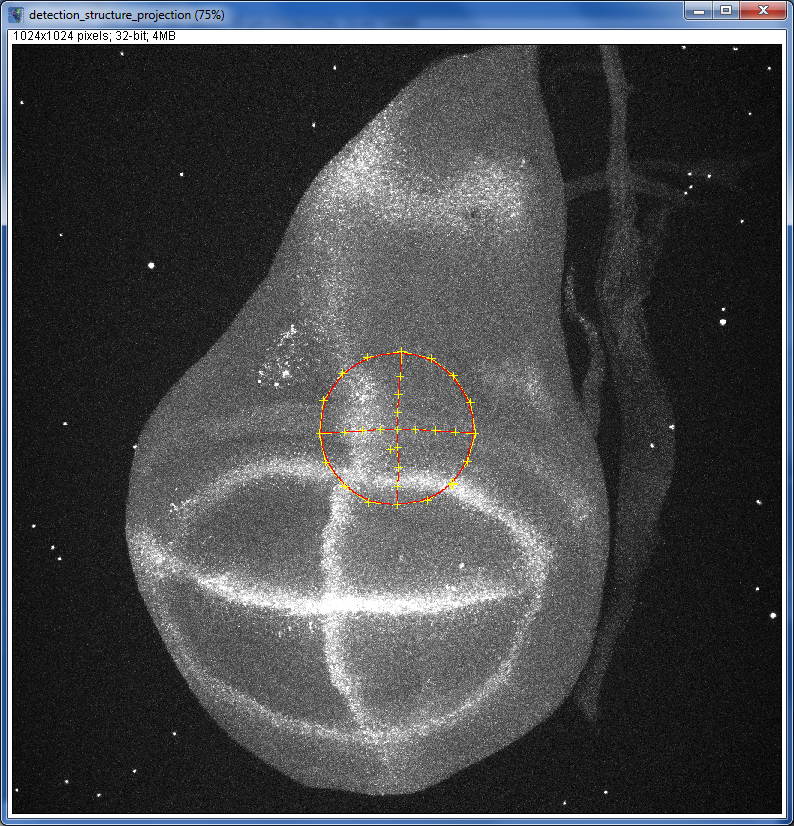
\includegraphics[scale=0.3]{images/wingj_structure_manual.jpg}
\caption{\textbf{Manual structure detection.} \wingj provides tools to manually generate structure models, for instance when a given biological system (organism or organ) is not yet implemented in \wingj. After loading an image stack, click on \textit{Manual} from the main interface of \wingj to generate a generic model that can be then shaped to fit the desired structure. The relevant structure is defined by the red, smooth polygon. The control points of the parametric model are represented by yellow vertices '+'. Finally, click on the \textit{tick mark} from the \textit{\ij toolbar} to validate the model (\sectionref{sec:structure_panel}).}
\label{fig:wingj_structure_manual}
\end{figure}

\textbf{Tip}: Hold \textit{Shift} to move the structure. The \textit{\ij toolbar} includes additional tools to rotate and scale the structure (\sectionref{sec:edit_structure_before_validation}).\\

\textbf{Tip}: To manually define a structure model, start by translating, rotating, and scaling the generic model to match roughly the target structure, then move the individual control points to locally modify the shape of the model.

% ===============================================================================
\section{Opening structure models from files}\label{sec:structure_import}
Click on \textit{Import} from the main interface of \wingj to import a structure model previously saved to file.

%  (wing pouch and embryo structure models are exported in XML format).

% If the step-by-step method failed or if no confocal images are available to provide information about the contour of the structure and the D/V and A/P boundaries, it is possible to manually define the structure by clicking on \textit{Manual}. The structure can then be modified as described in Section \ref{sec:fine-tuning}. To speed up the manual detection, you can drag-and-drop the generic structure by pressing MAJ key to center if with the effective structure. Fig. \ref{fig:structure_manual_2} shows the default generic structure which is displayed which is displayed right after clicking on \textit{Manual}.

% \begin{figure}[h!]
% \centering\includegraphics[width=12cm]{figures/structure_manual}
% \caption{Manual detection of the \textit{Drosophila} wing structure. A single vertex (yellow cross) is displayed at the North-East location of the default cross center. This vertex should be placed close to the Dorsal extremity of the D/V boundary to enable WingJ to correctly identify the orientation of the wing.}
% \label{fig:structure_manual_2}
% \end{figure}